 \documentclass[oneside,a4paper,12pt]{book}
%\pagestyle{headings}
\frontmatter

%=============================================================================

\usepackage{amsthm}
\usepackage{xspace}
\usepackage{float}
\usepackage{ifthen}
\usepackage{amsbsy}
\usepackage{amssymb}
\usepackage{balance}
\usepackage{booktabs}
\usepackage{graphicx}
\usepackage{rotating}
\usepackage{multirow}
\usepackage{needspace}
\usepackage{microtype}
\usepackage{bold-extra}
\usepackage{geometry}
\usepackage{varioref}
\usepackage{xcolor}
\usepackage{textcomp}
\usepackage{listings}
\usepackage[normalem]{ulem} %emphasize still italic
\usepackage{ucs}

% \usepackage[utf8]{inputenc}
% \usepackage[htt]{hyphenat}
\usepackage{times}
\usepackage{url}
\usepackage{alltt}
\usepackage{amsmath}
\usepackage{xfrac}
\usepackage{subfigure}
\usepackage{appendix}
\usepackage{stmaryrd}   % for the \shortuparrow
\usepackage[utopia]{quotchap}

\usepackage{setspace}
\usepackage[numbers, sort&compress]{natbib}
\usepackage{mdwlist}        % support for better spaced lists
% allows for temporary adjustment of side margins
\usepackage{chngpage}
\usepackage[normalem]{ulem} 

% lina entered
\usepackage{indentfirst}
\usepackage[parfill]{parskip}
\usepackage[bottom]{footmisc}

\usepackage[T1]{fontenc}
\usepackage{caption}
\usepackage{booktabs}
\usepackage{siunitx}


\setlength{\parindent}{1.5em}

% constants

\newcounter{qcounter}

% commands
\newcommand{\n}{$\cdot$}
\newcommand{\y}{\checkmark}
\newcommand{\subscript}[1]{$_{\textrm{\footnotesize{#1}}}$}
\newcommand{\superscript}[1]{$^{\textrm{\footnotesize{#1}}}$}
\newcommand{\vertical}[1]{\raisebox{-4em}{\begin{sideways}{#1}\end{sideways}}}
\newcommand\tab[1][1cm]{\hspace*{#1}}

\usepackage{boxedminipage}

\newboolean{showedits}
\setboolean{showedits}{true} % toggle to show or hide edits
\ifthenelse{\boolean{showedits}}
{
       \newcommand{\ugh}[1]{\textcolor{red}{\uwave{#1}}} % please rephrase
       \newcommand{\ins}[1]{\textcolor{blue}{\uline{#1}}} % please insert
       \newcommand{\del}[1]{\textcolor{red}{\sout{#1}}} % please delete
       \newcommand{\chg}[2]{\textcolor{red}{\sout{#1}}{\ra}\textcolor{blue}{\uline{#2}}} % please change
}{
       \newcommand{\ugh}[1]{#1} % please rephrase
       \newcommand{\ins}[1]{#1} % please insert
       \newcommand{\del}[1]{} % please delete
       \newcommand{\chg}[2]{#2}
}


% ============================================================================
% Put edit comments in a really ugly standout display

\usepackage{xcolor}
\usepackage[normalem]{ulem}
\newcommand{\ra}{$\rightarrow$}
\usepackage{amssymb}

% comments \nb{label}{color}{text}
\newboolean{showcomments}
\setboolean{showcomments}{true}
%\setboolean{showcomments}{false}
\ifthenelse{\boolean{showcomments}}
{\newcommand{\nb}[3]{
  {\colorbox{#2}{\bfseries\sffamily\scriptsize\textcolor{white}{#1}}}
  {\textcolor{#2}{\sf\small$\blacktriangleright$\textit{#3}$\blacktriangleleft$}}}
    \newcommand{\version}{\emph{\scriptsize$-$Id$-$}}
%	 \newcommand{\ugh}[1]{\textcolor{red}{\uwave{#1}}} % please rephrase
%	 \newcommand{\ins}[1]{\textcolor{blue}{\uline{#1}}} % please insert
%	 \newcommand{\del}[1]{\textcolor{red}{\sout{#1}}} % please delete
%	 \newcommand{\chg}[2]{\textcolor{red}{\sout{#1}}{\ra}\textcolor{blue}{\uline{#2}}} % please change
	 \newcommand{\chk}[1]{\textcolor{ForestGreen}{#1}} % changed, please check
	}
{\newcommand{\nb}[3]{}
  \newcommand{\version}{}
  \newcommand{\chk}[1]{} % changed, please check
  }
\newcommand\nm[1]{\nb{NM}{violet}{#1}} % add more author macros here
\newcommand\lt[1]{\nb{LT}{orange}{#1}}


% ============================================================================
% Make quotes be italic
\renewenvironment{quote}
    {\list{}{\rightmargin\leftmargin}%
     \item\relax\begin{it}}
    {\end{it}\endlist}

\newcommand{\ttimes}{\ensuremath{\times}}

%=============================================================================

\newcommand{\needlines}[1]{\Needspace{#1\baselineskip}}

% source code
\usepackage{xcolor}
\usepackage{textcomp}
\usepackage{listings}
\definecolor{javared}{rgb}{0.6,0,0} % for strings
\definecolor{javagreen}{rgb}{0.25,0.5,0.35} % comments
\definecolor{javapurple}{rgb}{0.5,0,0.35} % keywords
\definecolor{javadocblue}{rgb}{0.25,0.35,0.75} % javadoc

\renewcommand{\lstlistingname}{Code}% Listing -> Algorithm
\renewcommand{\lstlistlistingname}{List of \lstlistingname s}% List of Listings -> List of Algorithms

\lstnewenvironment{Java}[1][]
{\lstset{
	language=Java,
	basicstyle=\footnotesize\ttfamily,
	keywordstyle=\color{javapurple}\bfseries,
	stringstyle=\color{javared},
	commentstyle=\color{javagreen},
	morecomment=[s][\color{javadocblue}]{/**}{*/},
	numbers=left,
	numberstyle=\tiny\color{black},
	stepnumber=1,
	numbersep=10pt,
	tabsize=4,
	showspaces=false,
	showstringspaces=false,
	breaklines=true,
	captionpos=b,
	xleftmargin=2em,
	framexleftmargin=1.5em,
	frame=single,
	#1
}}
{}


\lstnewenvironment{JVMIS}[1][]
{\lstset{
	language=JVMIS,
	basicstyle=\footnotesize\ttfamily,
	keywordstyle=\color{javagreen}\bfseries,
	stringstyle=\color{javared},
	commentstyle=\color{javagreen},
	morecomment=[s][\color{javadocblue}]{/**}{*/},
	numbers=none,
	numberstyle=\tiny\color{black},
	stepnumber=1,
	numbersep=10pt,
	tabsize=4,
	showspaces=false,
	showstringspaces=false
	breaklines=true,
	captionpos=b,
	xleftmargin=2em,
	framexleftmargin=1.5em,
	frame=single,
	#1
}}
{}


\definecolor{codegray}{gray}{0.9}
\newcommand{\code}[1]{
	\colorbox{codegray}
	{\texttt{#1}}
}

%----------------------------------------------------------------------------
% references
\newcommand{\tabref}[1]{\hyperref[{tab:#1}]{Table~\ref*{tab:#1}}}
\newcommand{\figref}[1]{\hyperref[{fig:#1}]{Figure~\ref*{fig:#1}}}
\newcommand{\secref}[1]{\hyperref[{sec:#1}]{Section~\ref*{sec:#1}}}
\newcommand{\subsecref}[1]{\hyperref[{subsec:#1}]{Subsection~\ref*{subsec:#1}}}
\newcommand{\lstref}[1]{\hyperref[{lst:#1}]{Listing~\ref*{lst:#1}}}
\newcommand{\charef}[1]{\hyperref[{ch:#1}]{Chapter~\ref*{ch:#1}}}
\newcommand{\coderef}[1]{\hyperref[{code:#1}]{Code~\ref*{code:#1}}}
\newcommand{\bytecoderef}[1]{\hyperref[{bytecode:#1}]{Bytecode~\ref*{bytecode:#1}}}
\newcommand{\algref}[1]{\hyperref[{alg:#1}]{Algorithm~\ref*{alg:#1}}}
\newcommand{\boxref}[1]{\hyperref[{box:#1}]{Box~\ref*{box:#1}}}

%----------------------------------------------------------------------------

% abbreviations
\tracingcolors 4
\setcounter{tocdepth}{3}
\setcounter{secnumdepth}{3}
\newcommand{\ie}{\emph{i.e.,}\xspace}
\newcommand{\eg}{\emph{e.g.,}\xspace}
\newcommand{\etc}{\emph{etc.}\xspace}
\newcommand{\etal}{\emph{et al.}\xspace}


\newcommand{\newevenside}{
	\ifthenelse{\isodd{\thepage}}{\newpage}{
	\newpage
        \phantom{placeholder} % doesn't appear on page
	\thispagestyle{empty} % if want no header/footer
	\newpage
	}
}

\def\stretchfactor{1}
\newcommand{\mychapter}[1]{\setstretch{1}
    \chapter{#1}\setstretch{\stretchfactor}}

%----------------------------------------------------------------------------
\newcommand{\lessSpace}{\vspace{-1em}}
\DeclareGraphicsExtensions{.pdf,.png}
\graphicspath{{images/}}
\newcommand{\fig}[4]{
	\begin{figure}[#1]
		\centering
		\includegraphics[width=#2\textwidth]{#3}
		\lessSpace
		\caption{\label{fig:#3}#4}
	\end{figure}}

% ===========================================================================

%:CONFIGURE THIS

\newcommand{\thesistitle}{Where does this null come from ?}
\newcommand{\thesisauthor}{Lina Tran}
\newcommand{\thesisauthorOrigin}{Biel/Bienne BE, Switzerland}
\newcommand{\thesisleiter}{Prof.\ Dr.\ Oscar Nierstrasz}
\newcommand{\thesisasst}{	\begin{center}
														Research assistant Nevena Milojkovi\'{c}\\
														Research assistant Boris Spasojevi\'{c}
													\end{center}}
\newcommand{\thesisurl}{http://scg.unibe.ch/}
\newcommand{\thesissubtitle}{An Approach to show the exact location where a value was referenced to null}
\newcommand{\thesisdate}{31. July 2016}

% ===========================================================================

\usepackage[ colorlinks=true, urlcolor=black, linkcolor=black,
			citecolor=black, bookmarksnumbered=true, bookmarks=true,
			plainpages=false,
			pdftitle={\thesistitle}, pdfauthor={\thesisauthor},
			pdfsubject={\thesissubtitle}, pdfpagelabels]{hyperref}

\newcommand{\hrref}[2]{\hyperref}
% ===========================================================================
% ===========================================================================


% D O C U M E N T
% % % % % % % % % % % % % % % % % % % % % % % % % % % % % % % % % %
\begin{document}

% T I T L E
% % % % % % % % % % % % % % % % % % % % % % % % % % % % % % % % % %
\begin{titlepage}  
  \begin{center}  
  
  \begin{figure}[t]  
  \vspace*{-2cm}        % to move header logo at the top 
  \center{
\includegraphics[scale=0.5]{logos/UNI_Bern.png}}
  \vspace{1in}     
  \end{figure}

    \thispagestyle{empty}
    
    {\bfseries\Huge \thesistitle \par
    \Large \vspace{0.1in} \thesissubtitle \par}

    \vspace{0.3in} 
    \LARGE{\textbf{Bachelor Thesis} \\}
    \vspace{0.4in}

    {\Large \thesisauthor \par from \par \thesisauthorOrigin}
    
    \vspace{0.3in}
    {\Large Faculty of Science \\
            University of Bern \par}
    \vspace{0.3in}
    {\Large \thesisdate \par}
    \vspace{0.3in}
    %Leiter der Arbeit: \par
   {\Large \thesisleiter} \par
      {\Large \thesisasst} \par
   \vspace{0.1in}
    {\Large Software Composition Group \par Institute for Computer Science \par University of Bern, Switzerland \par}
  

  %\vspace{0.5in}
 
 

  \end{center}

\end{titlepage}


% A B S T R A C T
% % % % % % % % % % % % % % % % % % % % % % % % % % % % % % % % % %
\chapter*{\centering Abstract}
\begin{quotation}
\noindent 
A previous study found out that \ugh{NullPointerExceptions}\brs{not sure if we can use NullPointerException as a word. We need to double check that} are the most frequently occurring and the most difficult to debug exceptions in Java projects. They are difficult to debug because the developer is only provided with a stack trace to where the exception was thrown. This only gives insight into the effect of the fault but not into its cause.

The aim of the project is to provide the developer with an additional stack trace of where the variable that caused the NullPointerException was actually set to null. We attempt to achieve this goal by instrumenting java source code striving for a minimal execution overhead. 

By tracking the null assignments through static analysis and instrumentation of the bytecode we can achieve a more efficient debugging process after an occurrence of a NullPointerException. 
\end{quotation}
\clearpage


% C O N T E N T S 
% % % % % % % % % % % % % % % % % % % % % % % % % % % % % % % % % % % % % % % %
\tableofcontents

\mainmatter
%%%%%%%%%%%%%%%%%%%%%%%%%%%%%%%%%%
%%%% NEW CHAPTER %%%%%%%%%%%%%%%%%%%%%
%%%%%%%%%%%%%%%%%%%%%%%%%%%%%%%%%%
\chapter{Introduction}
\label{ch:introduction}
Nowadays, practically all Java developers are confronted with NullPointerExceptions in both big and small Java projects, whether it is for an enterprise or for private purposes. The seriousness of null dereferencing is apparent from the finding that 35\% of the conditional statements in open source Java projects are null checks which degrades the readability of code and of course has a negative impact on performance~\cite{Osma15a}. It is also considered the number one error Java programmers make\footnote{\url{http://www.javacoffeebreak.com/articles/toptenerrors.html}}.

NullPointerException is a commonly occurring RuntimeException in object-oriented languages. There is a special value \textit{null} that is assigned to pointers to indicate that the pointer does not point to an object. The cause of NullPointerExceptions is a method invocation on an object assigned the value null or an attempt to access a field. This object reference can be a local variable, an instance field, an element of a collection or a return value of a function. In Java Projects developers always have to deal with a huge amount of references which means there is a high probability that there will be a NullPointerException.

Now we will present two different situations in which a NullPointerException can be thrown.

\begin{Java}[caption={NullPointerException example - Method receiver. This code snippet is form JHotDraw project\protect\footnote{\url{http://www.jhotdraw.org/}}.}, label={code:npeExampleMethodReceiver}]
public void drop(DropTargetDropEvent dtde) {
	//...
	try {
		//...
		DNDFigures ff = (DNDFigures)DNDHelper.processReceivedData(DNDFiguresTransferable.DNDFiguresFlavor, dtde.getTransferable());
		//...
		Point theO = ff.getOrigin();
		//...
	}
	catch (NullPointerException npe) {
		npe.printStackTrace();
		//...
	}
	//...
}
\end{Java}

Lets say that in \coderef{npeExampleMethodReceiver} the variable at line 5 is assigned the null value by the return value of the function \code{DNDHelper.processReceivedData()}. So the method receiver (\code{ff} at line 7) is null and when a method is called on this object a NullPointerException is thrown. Because the the NullPointerException occurred in the \code{try\{\}} block the \code{catch\{\}} block right after it handles the exception. The stack trace only takes the developer to line 7 where the exception is caused but not to the real culprit which is the assignment at line 5. This is a very simple example and the easiest way to produce a NullPointerException\brs{it's really not a simple example, we might consider finding a simpler one}. The root of the NullPointerException is located in the same method.

\begin{Java}[caption={NullPointerException example - Field access. This code snippet is taken from JHotDraw project\protect\footnote{\url{http://www.jhotdraw.org/}} and slightly modified.}, label={code:npeExampleFieldAccess}]
public class DrawApplication extends JFrame implements DrawingEditor,
		PaletteListener, VersionRequester {
	//...
	private IconkitManager fManager;
	
	public void open() {
		open(createInitialDrawingView());
	}
	
	protected void open(final DrawingView newDrawingView) {
		//...
		setIconkit(createIconkit());
		//...
		setTool(new NullTool(this), "");
		//...
	}
		
	protected Iconkit createIconkit() {
		fManager = getIconkitManager();
		//...
	}
	
	public void setTool(Tool t, String name) {
		//...
		fManager.getComponent();
		//...
	}
	//...
}
\end{Java}

With the method invocations in the method \code{open()} at line 10 the class instance \code{fManager} (line 4) is initialized by invoking the \code{createIconkit()} method at line 12 and is accessed at a later point. Suppose the instance field \code{fManager} is set to null by the function \code{getIconkitManager()} at line 19 when the method \code{createIconkit()} is executed. Later at line 14 the function \code{setTool()} is invoked which attempts an access to the field \code{fManager} that has a value of null. That means a NullPointerException is thrown at line 25 with the stack trace shown in \boxref{stackTrace} :

\begin{figure}[H]
\renewcommand\figurename{Box}
	\begin{boxedminipage}{\textwidth}
		\color{cadmiumred}
		Exception in thread "main" \textcolor{blue}{java.lang.NullPointerException}\newline
		\tab at org.jhotdraw.application.DrawApplication.setTool(\textcolor{blue}{DrawApplication.java:25})\newline
		\tab at org.jhotdraw.application.DrawApplication.open(\textcolor{blue}{DrawApplication.java:14})\newline
		\tab at org.jhotdraw.application.DrawApplication.open(\textcolor{blue}{DrawApplication.java:7})\newline
	 \tab ...
	\end{boxedminipage}
	\caption{Stack trace of a NullPointerException.}
	\label{box:stackTrace}
\end{figure}

In \boxref{stackTrace} we can see that the stack trace does not track to the root of the NullPointerException. We call the location where the variable was assigned the null value the root of an exception (in our case a NullPointerException). That means the Java developer has to debug to find the exception root.

All too often programmers states that they are trying to fix bugs or have spent a lot of time fixing them. Of course not all of the bugs are NullPointerExceptions but there could be few of them. If there would be a way to minimize the time fixing exceptions and allow to work more efficiently, projects would progress much faster.\nm{Rewrite: yes, developers deal with a lot of problems caused by null pointer exception, and you should find some paper to reference that.}\lt{can't find papers!}\brs{skipped this paragraph, let's sync}

At this point we would like to introduce our project named \textit{\textbf{NullSpy}} which supports the developers in situations discussed previously. In other words its main goal is to take a step on minimizing the debugging time. The intention behind NullSpy is to present the developers the exact location of the null assignment next to the ordinary stack trace.

In this thesis we explain how the goal mentioned above is achieved and we also discuss the challenges, the limitations and performance impact of the approach.

\chapter {Technical Background}
\label{ch:technicalBackground}

This chapter provides a short overview of technologies used in the implementation of NullSpy.

\section{Javassist}
\label{sec:javassist}
\textit{Javassist} or \textit{Java Programming Assistant}\footnote{\url{http://jboss-javassist.github.io/javassist/}}~\cite{Chib00}~\cite{Chib03}, a subproject of Jboss, is a class library which enables manipulation of the Java bytecode. Since 1999 it is used as an engineering toolkit in a broad domain, and is still being extended by Shigeru Chiba. It enables developers to manipulate Java bytecode in a simplified way. Examples of this manipulation include defining a new class at runtime or modifying a class file when it is loaded by the JVM. All manipulations are performed at load-time through a provided class loader. A tutorial for using Javassist\footnote{\url{http://jboss-javassist.github.io/javassist/tutorial/tutorial.html}} is available online and was used as a starting point for this work.

\begin{figure}[H]
\centering
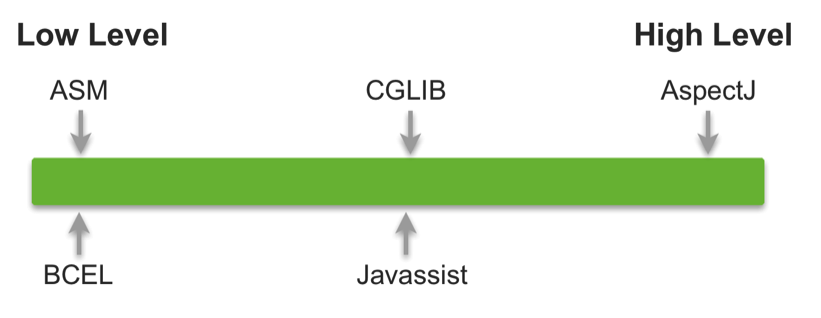
\includegraphics[width=0.8\linewidth]{javassistLevel}
\caption{Bytecode modification levels.}
  \label{fig:bytecodeModificationLevels}
\end{figure}

Unlike many other libraries Javassist offers two levels of API: \textbf{source}-level and \textbf{bytecode}-level (See \figref{bytecodeModificationLevels}\footnote{Figure taken from \href{https://blog.newrelic.com/2014/09/29/diving-bytecode-manipulation-creating-audit-log-asm-javassist/}{blog.newrelic.com}.}). Using the source-level API, the user can edit a class file without any familiarity with the specifications of the Java bytecode. Knowledge of the Java language is enough since the API is designed only with the vocabulary of Java. On this level the programmer has to write Java source code and Javassist compiles it automatically. The bytecode level allows the user to modify classes by modifying the bytecode directly.

At this point, let us look at a small example of how the bytecode manipulation works.

\begin{Java}[caption={Javassist example. This example is taken from the Javassist tutorial.}, label={code:javassistExample}][H]
ClassPool pool = ClassPool.getDefault();
CtClass cc = pool.get("test.Rectangle");
cc.setSuperclass(pool.get("test.Point"));
cc.writeFile();
\end{Java}

\begin{enumerate}
	\item First a \textit{ClassPool} object that controls bytecode modification with Javassist is obtained. With the \textit{ClassPool} a class file (``.class'') can be read on demand for constructing a \textit{CtClass} object.
	
	\item The class \textit{CtClass} (compile-time class) represents the class file meaning that all manipulations are performed on the \textit{CtClass} object. We obtain a reference to the \textit{CtClass} object representing the \code{test.Rectangle} class by invoking the \code{get()} method on the \textit{ClassPool} instance.
	
	\item In this example the superclass of \code{test.Rectangle} is simply changed to \code{test.Point}.
	\item Once the bytecode modification is done, the method call \code{writeFile()} on the instance of \textit{CtClass} is necessary to make sure that the changes are reflected on the original class file.
\end{enumerate}
 
\begin{figure}[H]
\centering
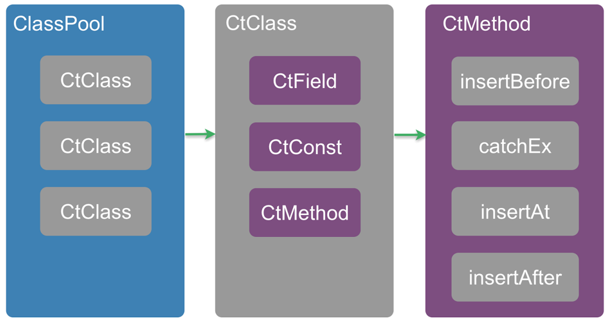
\includegraphics[width=0.8\linewidth]{javassistModules}
\caption{Javassist modules.}
  \label{fig:javassistModules}
\end{figure}

\figref{javassistModules}\footnote{Figure taken from \href{https://blog.newrelic.com/2014/09/29/diving-bytecode-manipulation-creating-audit-log-asm-javassist/}{blog.newrelic.com}.} gives an overview of how the main part of bytecode manipulation with Javassist is built up. The \textit{ClassPool} is simply a container of multiple \textit{CtClasses}. As described before \textit{CtClass} represents class files on which modifications are done. Like typical classes, it can hold compile-time fields, constants or methods. Javassist is capable of adding or modifying classes, behaviors, fields, method invocations, local variables \etc But in our case we mainly address the manipulation of behaviors. It is possible to insert additional source code at the beginning of the method body or at the end or at a specific line. The next example shows how to add code using Javassist.

\begin{Java}[caption={Initial code.}, label={code:initialCode}][H]
public static void main(String[] args) {
	System.out.println("This is an example class.");
}
\end{Java}

\renewcommand\lstlistingname{Bytecode}
\begin{JVMIS}[caption={Initial bytecode.}, label={bytecode:initialBytecode}, breaklines=true][H]
public static void main(java.lang.String[]);
  0: getstatic     #16	// Field java/lang/System.out:Ljava/io/PrintStream;
  3: ldc           #22	// String This is an example class.
  5: invokevirtual #24	// Method java/io/PrintStream.println:(Ljava/lang/String;)V
  8: return
\end{JVMIS}

We want to add one line of code at the beginning of \coderef{initialCode}. \bytecoderef{initialBytecode} is the corresponding bytecode of \coderef{initialCode}.

\renewcommand\lstlistingname{Code}
\begin{Java}[caption={Instrumentator.}, label={code:instrumentator}][H]
public class Instrumentator {
	public static void main(String[] args) throws NotFoundException,
			CannotCompileException, FileNotFoundException, IOException {
		ClassPool pool = ClassPool.getDefault();
		CtClass cc = pool.get("insertJavaCodeExample.ExampleClass");

		CtBehavior behavior = cc.getDeclaredMethod("main");
		behavior.insertBefore("System.out.println(\"This is the inserted code.\");");

		ClassFile classFile = cc.getClassFile();
		String destinationPath = args[0] + "\\ExampleClassInstrumented.class";
		classFile.write(new DataOutputStream(new FileOutputStream(
				destinationPath)));
	}
}
\end{Java}

With \coderef{instrumentator} we obtain a \textit{CtClass} object \code{cc} at line 5 which represents the class to be modified. At line 7 we get the method we want to modify by adding some source code: \code{System.out.println(``This is the inserted code.'');}. Javassist takes a \textit{java.lang.String} object, compiles it automatically and adds it into the bytecode at the specified location, in our situation at the beginning of the \code{main()} method. The modified class is then stored at a destination folder we chose (line 12).

Below the result, how the \code{main()} method looks like after the modification. At line 2 we see the inserted code. 

\begin{Java}[caption={Instrumented code: Decompiled with JAD (\secref{jad})}, label={code:instrumentedCodeDecompiled}][H]
public static void main(String args[]) {
	System.out.println("This is the inserted code.");
	System.out.println("This is an example class.");
}
\end{Java}

And of course the \bytecoderef{modifiedBytecode} has changed since Javassist added additional bytecode. The pc-interval [0,3,5] represents the added code.

\renewcommand\lstlistingname{Bytecode}
\begin{JVMIS}[caption={Modified bytecode.}, label={bytecode:modifiedBytecode}, breaklines=true][H]
public static void main(java.lang.String[]);
  0: getstatic     #16 	// Field java/lang/System.out:Ljava/io/PrintStream;
  3: ldc           #35	// String This is the inserted code.
  5: invokevirtual #24	// Method java/io/PrintStream.println:(Ljava/lang/String;)V
  8: getstatic     #16	// Field java/lang/System.out:Ljava/io/PrintStream;
 11: ldc           #22	// String This is an example class.
 13: invokevirtual #24	// Method java/io/PrintStream.println:(Ljava/lang/String;)V
 16: return
\end{JVMIS}

\brs{not sure how the remainder here is relevant, please just give a nice example of some source code, how one would add code to it using javasist and the result} \lt{ganzer paragraph weg?}
Next to these options even a \textit{catch block} can be added. The difference between \code{insertAfter()} and \code{addCatch()} is insertAfter inlines some code right before every return instruction in the method body and addCatch adds a catch clause to the method which handles an exception thrown in the body. So the catch clause is always positioned at the end of the method body. In \figref{insertionCodeExample} below a small insertion example is demonstrated.

\begin{figure}[H]
\centering
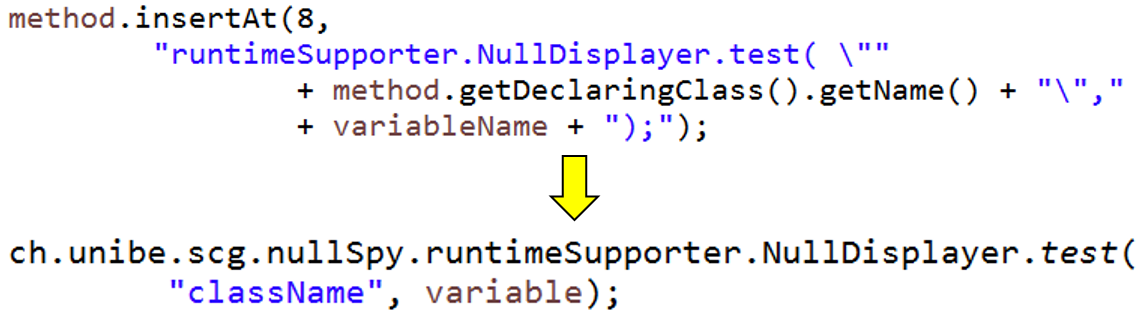
\includegraphics[width=0.9\linewidth]{insertionCodeExample}
\caption{Inserting code example.}
  \label{fig:insertionCodeExample}
\end{figure}

\section{JAD}
\label{sec:jad}
Java Decompier (JAD)\footnote{\url{https://sourceforge.net/projects/jadclipse/}} is a decompiler and a Eclipse plugin for the programming language Java. A decompiler is a program that takes an executable file as input, and attempts to create a high level, compatible source file. If the source file is compiled again, it will produce an executable program that behaves the same way as the original one. It is often used in software reverse engineering.

The example \bytecoderef{jad} is decompiled by JAD and the result is the source code right under the example. It is also a good opportunity to present how bytecode looks like.

\begin{JVMIS}[caption={Bytecode example.}, label={bytecode:jad}, breaklines=true]
public void itemStateChanged(java.awt.event.ItemEvent e);
  0  aload_1 [e]
  1  invokevirtual java.awt.event.ItemEvent.getStateChange()...
  4  iconst_1
  5  if_icmpne 22
  8  aload_0 [this]
  9  getfield org.jhotdraw.applet.DrawApplet$1.this$0 : ...
 12  aload_1 [e]
 13  invokevirtual java.awt.event.ItemEvent.getItem() : ...
 16  checkcast java.lang.String [33]
 19  invokevirtual org.jhotdraw.applet.DrawApplet....
 22  return
Line numbers:
 [pc: 0, line: 213]
 [pc: 8, line: 214]
 [pc: 22, line: 216]
Local variable table:
 [pc: 0, pc: 23] local: this index: 0 type: new org...
 [pc: 0, pc: 23] local: e index: 1 type: java.awt.event...
Stack map table: number of frames 1
 [pc: 22, same]
\end{JVMIS}

\renewcommand\lstlistingname{Code}
\begin{Java}[caption={Decompiled bytecode.}, label={code:decompiledBytecode}]
public void itemStateChanged(ItemEvent e) {
	if(e.getStateChange() == 1)
	loadDrawing((String)e.getItem());
}
\end{Java}

JAD is in no way a dependency of NullSpy but it was a big help during the implementation phase. Since after running NullSpy on a project only the modified bytecode is available. The use of JAD is for the sake of debugging Nullspy; to check whether the modification by Javassist, e.g. inserting source code, has succeeded. Another way to check the result for correctness is looking at bytecode itself but that would have taken a lot more effort and time.

\chapter{NullSpy}
As explained in \charef{introduction}, this project is about providing the user with an additional stack trace containing the information on where the null is assigned to the variable that caused the NullPointerException. In short, it shows the developer the exact location of where a method receiver\brs{I'm not sure method receiver is the right jargon (Ausdrucksweise) for java. we need to check} or a field (in a field access case) was assigned null.

Here we give a short overview of how we implemented the core of NullSpy. We will also address the challenges (\secref{challenges}) we encountered during the implementation as well as the limitations of the tool (\secref{limitations}).

\section{High Level Overview}
\label{sec:highLevelOverview}
The general approach of NullSpy is to statically analyze a project and instrument the bytecode. \lt{In NullSpy we are working with the value of variable. Since ...} \nm{You should add a sentence or two to explain this more. Why statical
analysis? Why adding bytecode?} \ugh{We add bytecode to check on every variable for its value and extract information (name, line number etc.) about it if necessary. Another reason is to get information about method receivers} (\boxref{methodReceiverInfo}). \ugh{To know where exactly they are placed in source code we need to statically examine the code and insert the bytecode at the right place.}\brs{this part carries no information at all. I have no idea what you wanted to say here and why. are we not talking about high level overview here? \ie the architecture etc.?} 

NullSpy first loads the project that we wish to instrument. Loading the project to NullSpy addressed only, the compiled class files of the project, which means the project source code does not have to be imported into the programming environment, e.g. Eclipse. Simultaneously at load time as each class file is loaded the bytecode is modified as described \secref{lowLevelOverview}.

Once the project modification is done it is stored in a destination folder that the user has chosen before\brs{How? it might be a good idea to discuss the command line arguments}. This means that the updated bytecode will be stored in another location, keeping the original class files intact.

\begin{figure}[H]
\centering
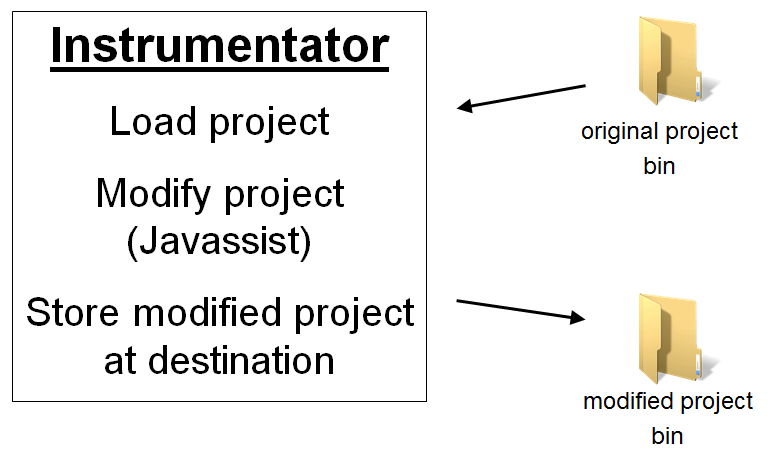
\includegraphics[width=0.5\linewidth]{highLevelOverview}
\caption{Modification overview.}
  \label{fig:highLevelOverview}
\end{figure}
\brs{\url{http://www.merriam-webster.com/dictionary/instrumentator}. Also, you could break up the one block in to separate phases to make it more clear what happens.} \lt{verstehe nicht}

Of course the original project can be replaced by the modified one too. But the developer has to think carefully about it because once replaced, the additional bytecode stays there and the execution time is slightly different than it was before. To get rid of the additional bytecode, the developer has to recompile the source code to get the original class files when needed. This has to be done every time when NullSpy is used on the project.

\section{Low Level Overview}
\label{sec:lowLevelOverview}

\ugh{NullSpy only handles the unhandled NullPointerException, meaning the main method of a project is wrapped with a \textit{catch block} where the NPE is treated. The idea in this \textit{catch block} is to load the data about the assignments and about the method receiver to compare them with each other. NullSpy will add other classes to the project which manage the added bytecode. One of those classes keeps \textit{HashMaps} in which data about assignments is stored. They are stored in HashMaps because each variable has a unique key. Next time if a variable is assigned with another value than null, its entry in the HashMap is deleted since it cannot cause a NullPointerException anymore. The data about the method receiver which is loaded is stored in an external \textit{csv} file for performance reasons.}

\ugh{In a NullPointerException situation the developer is provided with the stack trace with which he/she can extract the information about the line number and the Java class name of where the NullPointerException occurred. Those data serves as a search criteria for further actions. We look these two information up in the file about the method receiver data. On a match more details about the method receiver can be read out. With this method receiver entry information we search for its assignment location which can be found in the HashMaps containing the details about all null assignments. And finally, if an entry in the HashMaps is found which matches the information extracted before, the exact location of the null assignment is found. The result is providing the user with an additional stack trace link next to the usual one. Clicking on that link will take one directly to the NullPointerException root. So to be able to provide this function, data about the method receivers and variable assignments have to be collected initially.} 
\brs{you are all over the place here, talking about everything from wrapping main to hashmaps and csv files. It's confusing even to me. I think maybe we should get together and try to build up a structure for this chapter}

A NullPointerException can be thrown if a method call was performed on an object or we attempt to access a field which is assigned null. To keep it simple for further explanations we will only mention method receiver from now on instead of method receiver and field.\brs{again, not sure of method receiver is good jargon for java. In any case, we should define the term like this earlier, i like avoiding the ``method or field access'' every time}

To reach the goal of NullSpy we have to gather information about the method receiver. A list of what kind of information is needed about the method receiver can be found in \subsecref{methodReceiver}. As well information about the variable assignments has to be collected to know the exact location of the null assignments. The main idea behind NullSpy actually is to get information comparing those together when a NullPointerException occurs and if there is a hit during the comparison the location of the null assignment can be obtained easily.\brs{again, we need better structure here, I get you are trying to give an overview and then dig in to the specifics, but it's just too much details for an overview, and not enough to be clear}

To explain the approach we will go through an example. The \coderef{npeExampleMethodReceiver} serves as a good example\brs{phrasing aside, it's unacceptable to refer to the example from chapter 1 in chapter 3. do you expect the reader to scroll up and down to follow the example? Also, I skipped the remainder of this section, we need heavy refactoring to make this work, 2 pages of textual description is too hard to follow.}. One method receiver is located at line 7 with the name \code{ff}. We extract information from bytecode about it and store the result in an external csv file. Data like name, type, line number, behavior, class etc. are stored (full list: \boxref{methodReceiverInfo}). The next step is to find all assignments in the code and insert new bytecode right after the assignments. In the example two assignments are present, in line 5 and 7. To do something with them obviously we have to know them better, that is why we again extract data about the variables \code{ff} and \code{theO} and pass the gathered information further to the inserted code right before line 6 and line 8 starts. The new bytecode checks whether the variables are null and stores the information about the variable with null value in a HashMap. The name and type of the variable \code{ff}, the behavior name and its signature and much more are stored in the HashMap.

If a NullPointerException is thrown the \code{main()} method will catch it. From stack trace info like the line number 7, the method name \textit{``drop"} and its signature, and the class name are read out. The \code{main()} method loads the csv file about the method receivers and looks up those details extracted from the stack trace. There is an entry (data about \code{ff}) which matches those search criteria. From the entry we need the name, type etc. from the variable. Now the \code{main()} method looks up the data about the variable in the HashMaps of the variable assignments. In the HashMaps the \code{main()} method finds the record with the same information as the method receiver \code{ff}. This record contains the exact location where null was assigned to the variable \code{ff}. With the line number 5, the behavior name drop and class name X the link which points to the assignment location can be created and is added to the origin stack trace. With only a click on that link the root of the NullPointerException is exposed.

The implementation behind the NullSpy concept will be explained more thoroughly.

\subsection{Method Receiver Data Collection}
\label{subsec:methodReceiver}
Unfortunately, Javassist does not provide the function to directly get the method receiver. With the following algorithm we managed to get the method receiver. The algorithm contains following steps:

\begin{figure}[H]
\renewcommand\figurename{Algorithm}
	\begin{boxedminipage}{\textwidth}
		\begin{enumerate}
\itemsep8pt
      \item Getting pc-interval\brs{pc-interval? never mentioned before and now we need to get it?} of method invocation
      \item Storing all possible method receiver interval within the interval of step 1 into an ArrayList
			\item Getting the number of parameters, the method invocation takes
			\item Traversing back the ArrayList the amount of parameters obtained in step 3
			\item Result: method receiver interval
			\item Store variable name, type etc. into an external csv file
   \end{enumerate}
	\end{boxedminipage}
	\caption{Method receiver algorithm.}
	\label{alg:methodReceiverAlg}
\end{figure}

In step 1 we had big troubles getting the right interval of the method receiver because only by statically analyzing the bytecode it is unapparent where the method receiver is situated exactly. But more about the challenges in \subsecref{methodReceiverDifficulties}.

Statically analyzing bytecode for method receiver means looking for certain opcodes which matches all opcodes that matches with the regex \textit{``invoke.*"}. There are exactly five kinds of bytecode instruction: \textit{invokedynamic}, \textit{invokeinterface}, \textit{invokespecial}, \textit{invokestatic}, \textit{invokevirtual}. The invocation opcode invokedynamic facilitates the dynamic-typed languages\footnote{Language whose type checking is usually performed at runtime.} through dynamic method invocation. In our case it can be ignored because NullSpy only supports the static-typed language\footnote{Language whose type checking is performed at compile time.} Java.

In case of the \textit{invokestatic} instruction we do not have a method receiver. That is why NullSpy treats it extraordinary like ignoring it completely or wrap it as a possible method receiver when it is actually a parameter of a method invocation. In all other cases we normally use the algorithm to get the method receiver. The gathered data about method receivers are stored in an external \textit{csv} file due to performance and overhead minimization. The following list will list the information which is stored about the method receiver.

\begin{figure}[H]
\renewcommand\figurename{List}
	\begin{boxedminipage}{\textwidth}
		\begin{itemize}
		\itemsep8pt
    \item nr (method receivers are counted)
		\item lineNumber
		\item variableID (whether it is a local variable or a field)
		\item variableType
		\item isVariableStatic
		\item ClassWhereVariableIsAccessed
		\item behavior (method)
		\item behaviorSignature
		\item localVariableAttributIndex
		\item fieldDeclaringClassName
   \end{itemize}
	\end{boxedminipage}
	\caption{Method receiver information.}
	\label{box:methodReceiverInfo}
\end{figure}

\subsection{Variable Data Collection}
\label{subsec:variable}
While going through the bytecode attention is paid to some opcodes\footnote{Operation code: Machine language instruction.}. Right after each keyword that indicates a variable assignment we insert some bytecode. The inserted code represents a test method which tests whether the value of the assigned variable is null or not and store some information about it. Unlike in getting information about the method receiver in \subsecref{methodReceiver} the data about the variables are stored in a HashMap.

What kind of opcodes were NullSpy looking for? For instance or class/static variables the bytecode instruction \textit{getfield} and \textit{getstatic} were essential, for local variables the important opcodes were those which matches the regex \textit{``aload.*"}. Due to different types of variables and the limitation of Javassist gathering information about them was performed differently. Again getting the necessary data about the variables we encountered many difficulties which will be discussed in the \secref{challenges}.

\subsubsection{Local Variable}
\label{subsubsec:localVariable}
Unfortunately, Javassist does not provide any support for gaining information about local variables that is why getting the needed data we had to understand how bytecode is constructed. At this point we would like to give a small bytecode introduction.

\begin{figure}[H]
\centering
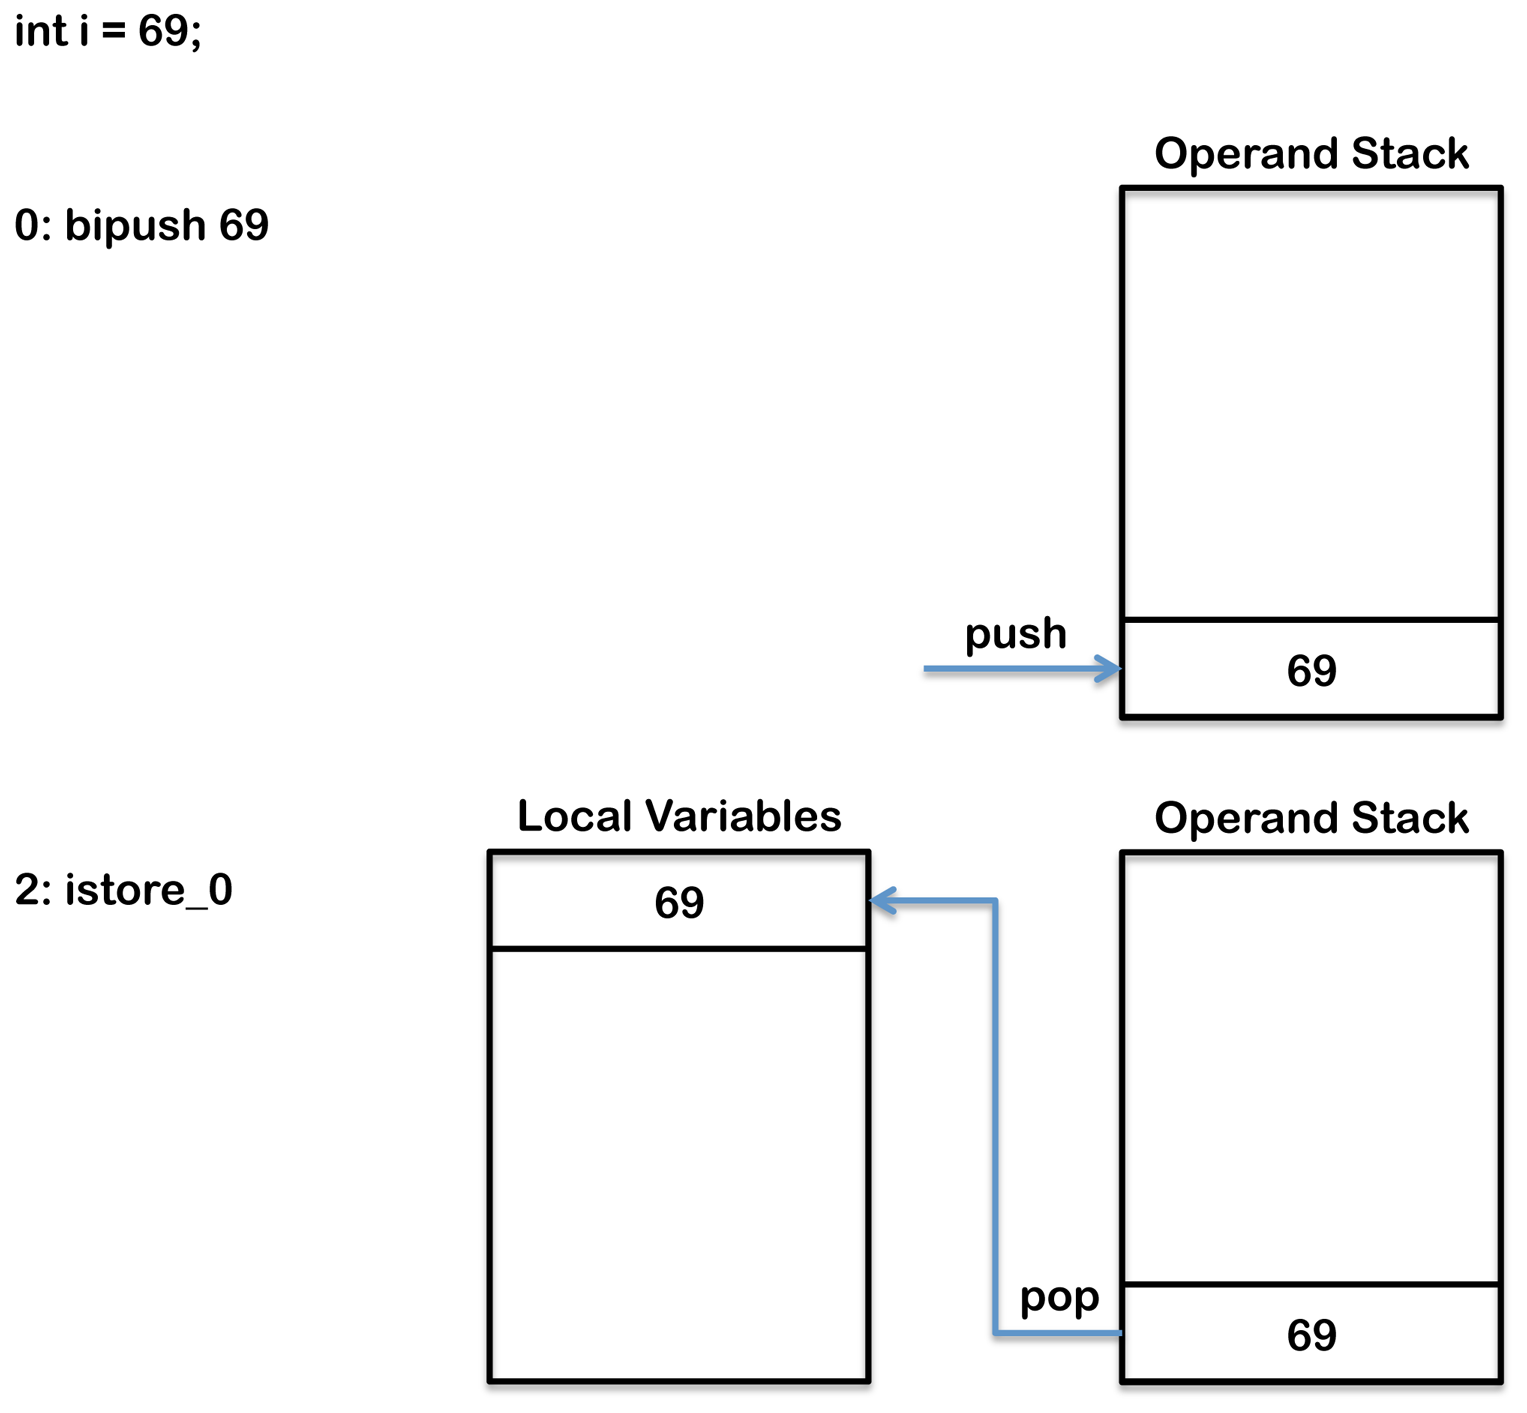
\includegraphics[width=0.8\linewidth]{localVarCreationBytecode}
\caption{Local variable creation\protect.}
  \label{fig:localVarCreationBytecode}
\end{figure}

If a local variable is created, the value assigned to it is pushed onto the operand stack as we can see in \figref{localVarCreationBytecode}\footnote{Figure taken from \href{http://blog.jamesdbloom.com/JavaCodeToByteCode_PartOne.html}{blog.jamesdbloom.com}.}. With the bytecode instruction \textit{``.*store.*"} the local variable is popped from the operand stack and stored into a local variable array slot. In which slot it is stored can be extracted from the instruction. Opcodes for storing local variables is composed of one, or in some cases two bytes. There are reserved machine commands for the first four local variables, index-linked from 0 to 3 and each of them contains one byte (astore\_0, astore\_1, astore\_2, astore\_3). If there is no slot number visible in the instruction, it indicates that the slot number is stored in the second byte from where it can be extracted. Next to storing the local variable loading it from the local variable array is possible to, but only with the local variable slot number.

With this short introduction understanding the local variable table should be easier. Each method of a class file contains a local variable table (see \bytecoderef{localVarTable}) with which many information can be read out of it, e.g. the lifespan of the local variable, what it is called, in which slot it is stored and what type it has.

\renewcommand\lstlistingname{Bytecode}
\begin{JVMIS}[caption={Local variable table.}, label={bytecode:localVarTable}]
Local variable table:
 [pc: 0, pc: 31] local: this index: 0 type: org.jhotdraw.samples...
 [pc: 0, pc: 31] local: newDrawing index: 1 type: org.jhotdraw...
 [pc: 5, pc: 31] local: d index: 2 type: java.awt.Dimension
 [pc: 22, pc: 31] local: newDrawingView index: 3 type: org.jhot...
\end{JVMIS}

We had to pay attention to be sure to get the right local variable. Every time when we bumped into the opcode \textit{``.*store.*"} we could only get its slot and the pc\footnote{Program counter/instruction pointer: A processor register that indicates where a computer is in its program sequence.} where it is situated in the bytecode sequence. In the earlier paragraph the lifespan of the local variable was mentioned, the importance behind this is as soon as the lifespan of one ends, the slot can be reused by the next instantiated local variable. This way, the local variable table could contain multiple entries with the same local variable slot.

\begin{JVMIS}[numbers=left, caption={Local variable table entries with same slot (line 5\&6).}, label={fig:localVarTableDuplicatedSlot}, breaklines=true]
Local variable table:
 [pc: 0, pc: 510] local: args index: 0 type: java.lang.String[]
 [pc: 24, pc: 510] local: m index: 1 type: isFieldOrLocalVar...
 [pc: 26, pc: 510] local: i index: 2 type: int
 [pc: 39, pc: 46] local: k index: 3 type: java.lang.Object
 [pc: 52, pc: 510] local: d index: 3 type: java.lang.Object}
 [pc: 71, pc: 510] local: d2 index: 4 type: java.lang.Object
\end{JVMIS}

After extracting the slot of the local variable we will get the first local variable table entry which contains that slot. If the pc of the local variable assignment is not included in the lifespan-pc-interval of the entry, the next entry with the same slot will be checked until both criteria (slot and pc) fits. Once those criteria are met we can be positive about having got the right local variable table entry to extract the information needed.

Next to the local variable table each methods of a class file also holds another attribute called line number attribute. This is the mapping table from pc to source code line number. Since encountering the storing keyword the pc is available , with help of it the line number can be easily obtained.

\begin{JVMIS}[caption={Line number table.}, label={code:lineNrTable}]
 Line numbers:
  [pc: 0, line: 26]
  [pc: 4, line: 27]
  [pc: 8, line: 29]
  [pc: 16, line: 30]
\end{JVMIS}

\subsubsection{Instance and Class/Static variables (Fields)}
\label{subsec:fields}
Although Javassist does not support the access to local variable it provides a way for fields. Javassist allows modifying an expression in a method body with the class \code{Javassist.expt.ExprEditor}. In our case we only want to extract some information about the fields instead of any modification, nevertheless this class can be used appropriately. What it does is to scan the bytecodes on instructions like \textit{``putfield"} or \textit{``putstatic"}.

There are only two instructions that indicates an access to a field, but there are actually many different types. To get the meaning of different types see the following list:

\begin{figure}[H]
\renewcommand\figurename{List}
	\begin{boxedminipage}{\textwidth}
		(\textbar\dots\textbar: put value on operand stack for assigning to a field)
\begin{enumerate}
\itemsep8pt
      \item aload\_0, \textbar\dots\textbar, putfield
      \item \textbar\dots\textbar, putstatic
			\item aload.*, \textbar\dots\textbar, putfield
			\item aload\_0, (getfield)+, \textbar\dots\textbar, putfield
			\item getstatic, (getfield)*, \textbar\dots\textbar, putfield
   \end{enumerate}
	\end{boxedminipage}
	\caption{Field keywords.}
	\label{box:fieldKeywords}
\end{figure}
	
Depending on the category the field belongs, different kind of information is stored. For fields 1-2 following information is needed and stored:

\begin{figure}[H]
\renewcommand\figurename{List}
	\begin{boxedminipage}{\textwidth}
		(\textbar\dots\textbar: put value on operand stack for assigning to a field)
\begin{itemize}
		\itemsep8pt
    \item fieldID (which is field or localVar)
		\item fieldname
		\item fieldType
		\item fieldDeclaringClassName (in which class it is instantiated)
		\item isFieldStatic
		\item fieldLineNumber
		\item startPosition (nonstatic: this; static: value loading bytecode for assigning to the field)
		\item storePosistion (putfield/putstatic)
		\item afterStorePosition (right before this pos additional bytecode is inserted)
		\item classWhereFieldIsAccessed (in this case the same as fieldDeclaringClassName)
		\item behavior (method where it is accessed)
		\item indirectVariable (null - explained immediately)
   \end{itemize}
	\end{boxedminipage}
	\caption{Variable information (I).}
	\label{box:variableInfo1}
\end{figure}

In NullSpy we call these fields \textit{``directFields"}. Reading \textit{``direct"} implicates that there must be something like \textit{``indirectFields"}, and that is right. As \textit{``indirectFields"} the fields 3-4 are numbered among. Everything before the instruction \textit{putfield} is termed as \textit{``indirectVariable"}. For those fields more data are needed to store for their identification. Nearly the same as above, except:

\begin{figure}[H]
\renewcommand\figurename{List}
	\begin{boxedminipage}{\textwidth}
\begin{itemize}
\itemsep8pt
      \item classWhereFieldIsAccessed (can be differend than fieldDeclaringClassName)
\item indirectVariable:
\begin{itemize}
\item indirectVariableName
\item indirectVariableType
\item indirectVariableDeclaringClassName
\item isIndirectVariableStatic
\item indirectVariableOpcode (to distinguisch if it is a localVariable or a field)
\end{itemize}
   \end{itemize}
	\end{boxedminipage}
	\caption{Variable information (II).}
	\label{box:variableInfo2}
\end{figure}

With a syntactic example we show how the instructions \textit{``putfield"} and \textit{``putstatic"} are used:

\renewcommand\lstlistingname{Code}
\begin{Java}[caption={Example: \textit{``putfield"} and \textit{``putstatic"}.}, label={code:instrExample}]
public class A {

	private B b = new B();
	private static B b2;

	public void x() {
		
		// |...|: value assigned
		
		// directFields
		this.b = ...; // aload_0, |...|, putfield
		b2 = ...; // |...|, putstatic

		B b3 = new B();
		
		// indirectFields
		b3.c = ...; // aload.*, (getfield)*, |...|, putfield
		b3.c.d = ...
		b.c = ...; // aload_0, (getfield)+, |...|, putfield
		b.c.d = ...;
		b2.c = ...; // getstatic, (getfield)*, |...|, putfield
		b2.c.d = ...;
	}
}

public class B {						
	public C c = new C();																
	...										
}				

public class C {
	public D d = new D();
	...	
}

public class D {
	...
}
\end{Java}

Once the bytecode is modified, the way to get the data of fields needs some adaptation (see \subsecref{variableDifficulties}).

\subsection{Bytecode Adaptation}
\label{bytecodeAdaptation}
Each time encountering a variable assignment we first extract the needed data and directly after this we adapt the class file by adding extra bytecode right after the assignment bytecode to check whether the variable is null or not. If it is null, the information collected before is stored either into the \textit{``localVariableMap"} or into a \textit{``fieldMap"} which are HashMaps.

The added bytecode represents a static method of a class named \code{VariableTester}\footnote{\label{package1}In package \emph{ch.scg.nullSpy.runtimeSupporter}.} which will be added to the modified project after class file modification is done. Depending on the kind of variable analyzed at the moment different bytecode is constructed, meaning different method with different parameter/variable data is added.

There were again some challenges we had to get over, like getting the wanted data after an instrumentation and entering the additional code in the right position of the bytecode sequence (\subsecref{bytecodeAdaptationDifficulties}).

Once we have gone through the bytecode of a Java class, the modified class files are stored in a destination directory as mentioned in \secref{highLevelOverview}. Next to the instrumentation supplementary supporter classes are added to the project. The most important ones are \code{VariableTester}\textsuperscript{\ref{package1}} which tests whether a variable is null or not and \code{NullDisplayer}\textsuperscript{\ref{package1}} which matches data and prints the location of a null assignment when a NullPointerException is thrown.

\section{Challenges}
\label{sec:challenges}
In this section we could like to give present some of the difficulties which occurred during the implementation of NullSpy.

\subsection{Obtaining Method Receiver Data Difficulties}
\label{subsec:methodReceiverDifficulties}
Aforementioned in \subsecref{methodReceiver} (\textit{Method Receiver Data Collection}) we were encountered with a persistent problem, namely getting the pc-interval of the method receiver when the interval covers multiple lines in source code. In many development environment the written code can be formatted automatically and as well manually. See following figures:

\begin{Java}[caption={Method invocation split in two lines example.}, label={code:4-1}, firstnumber=31]
Image image = Iconkit.instance().registerAndLoadImage(
	(Component)view, imageName);
\end{Java}

\renewcommand\lstlistingname{Bytecode}
\begin{JVMIS}[caption={Bytecode to \coderef{4-1}.}, label={bytecode:4-2}, breaklines=true]
 0  invokestatic org.jhotdraw.util.Iconkit.instance() : org.jhotdraw.util.Iconkit [22]
 3  aload_1 [view]
 4  checkcast java.awt.Component [28]
 7  aload_0 [this]
 8  getfield org.jhotdraw.samples.minimap.MiniMapDesktop.imageName : java.lang.String [14]
11  invokevirtual org.jhotdraw.util.Iconkit.registerAndLoadImage(java.awt.Component, java.lang.String) : java.awt.Image [30]
14  astore_2 [image]
\end{JVMIS}

\begin{JVMIS}[caption={Line number table/interval to \coderef{4-1}.}, label={bytecode:4-3}, breaklines=true]
[pc: 0, line: 31]
[pc: 3, line: 32]
[pc: 11, line: 31]
\end{JVMIS}


%\begin{figure}[H]
%\centering
%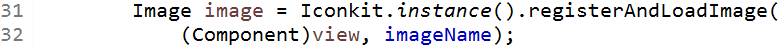
\includegraphics[width=\linewidth]{multipleLine/pic4-1}
%\caption{Method invocation split in two lines example.}
%  \label{fig:pic4-1}
%\end{figure}

%\begin{figure}[H]
%\centering
%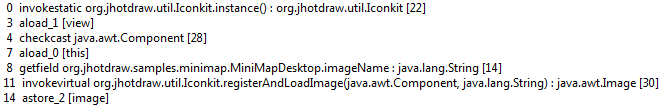
\includegraphics[width=\linewidth]{multipleLine/pic4-2}
%\caption{Bytecode to \figref{pic4-1}.}
%  \label{fig:pic4-2}
%\end{figure}

%\begin{figure}[H]
%\centering
%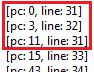
\includegraphics[width=0.3\linewidth]{multipleLine/pic4-3}
%\caption{Line number table/interval to \figref{pic4-1}.}
%  \label{fig:pic4-3}
%\end{figure}

Figure shows a normal method invocation which is split into two lines in source code. This cannot be figured out by just looking at the bytecode therefore the line number attribute (\coderef{lineNrTable}) has to be consulted too. There is no method receiver in the figure because the method receiver would contain a method invocation itself, what is not supported in NullSpy. Another method receivers NullSpy does not support are elements of collections due to complex structures that can be stored in the collections. But still it is a good example to show how the bytecode and the line number attribute for this looks like. Applying the (\algref{methodReceiverAlg}) for gathering data about method receivers in this situation looks as follows:

\begin{figure}[H]
\renewcommand\figurename{Algorithm}
	\begin{boxedminipage}{\textwidth}
		\begin{enumerate}
			\itemsep8pt
			\item pc-interval: \newline 0-11 (cut everything off what has nothing to do with the method invocation)
			\item ArrayList: \newline [0,[3,4],[7,8]]
			\item Number of parameters: \newline 2
			\item Traversing back the amount of parameters: \newline [7,8] (1) ; [3,4] (2)
			\item Result: \newline 0 (invokestatic) = possible method receiver
			\item Not storing it because NullSpy does not support this kind of method receiver
		\end{enumerate}
	\end{boxedminipage}
	\caption{Extract method receiver example.}
	\label{box:extractMethodReceiverExample}
\end{figure}

Only looking at bytecode is not enough, so we are looking at the line number attribute. Line number \textit{31} (\bytecoderef{4-3}) is listed twice, this indicates that the method invocation is split into multiple line in source code. The former declares the starting point of the interval and the latter the end of it. How to get the pc-interval will be presented shortly. But first take a look at more examples:

\renewcommand\lstlistingname{Code}
\begin{Java}[caption={Alternating line number example.}, label={code:3-1}, firstnumber=127]
Connector oldConnector = ((ChangeConnectionHandle.UndoActivity)
			getUndoActivity()).getOldConnector();
\end{Java}

\renewcommand\lstlistingname{Bytecode}
\begin{JVMIS}[caption={Bytecode to \coderef{3-1}.}, label={code:3-2}, breaklines=true]
47  aload_0 [this]
48  invokevirtual org.jhotdraw.standard.ChangeConnectionHandle.getUndoActivity() : org.jhotdraw.util.Undoable [72]
51  checkcast org.jhotdraw.standard.ChangeConnectionHandle$UndoActivity [76]
54  invokevirtual org.jhotdraw.standard.ChangeConnectionHandle$UndoActivity.getOldConnector() : org.jhotdraw.framework.Connector [142]
57  astore 7 [oldConnector]
\end{JVMIS}

\begin{JVMIS}[caption={Line number table/interval to \coderef{3-1}.}, label={code:3-3}, breaklines=true]
[pc: 47, line: 128]
[pc: 51, line: 127]
[pc: 54, line: 128]
[pc: 57, line: 127]
\end{JVMIS}

%\begin{figure}[H]
%\centering
%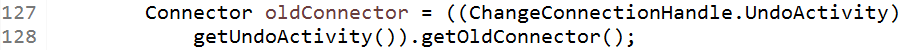
\includegraphics[width=\linewidth]{multipleLine/pic3-1}
%\caption{Alternating line number example.}
%  \label{fig:pic3-1}
%\end{figure}

%\begin{figure}[H]
%\centering
%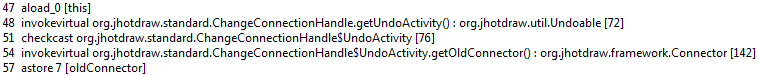
\includegraphics[width=\linewidth]{multipleLine/pic3-2}
%\caption{Bytecode to \figref{pic3-1}.}
%  \label{fig:pic3-2}
%\end{figure}

%\begin{figure}[H]
%\centering
%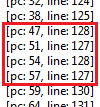
\includegraphics[width=0.3\linewidth]{multipleLine/pic3-3}
%\caption{Line number table/interval \figref{pic3-1}.}
%  \label{fig:pic3-3}
%\end{figure}

Special about this example is that the multiple line interval does not start with the smaller line number and end with the bigger one, apart from that it is alternated stored in the line number attribute.

\renewcommand\lstlistingname{Code}
\begin{Java}[caption={Nested interval example.}, label={code:2-1}, firstnumber=149]
for (int i = 0; i < ColorMap.size(); i++)
	choice.addItem(
		new ChangeAttributeCommand(
			ColorMap.name(i),
			attribute,
			ColorMap.color(i),
			this
		)
	);
\end{Java}

\renewcommand\lstlistingname{Bytecode}
\begin{JVMIS}[caption={Bytecode to \coderef{2-1}.}, label={code:2-2}, breaklines=true]
 8  iconst_0
 9  istore_3 [i]
10  goto 37
13  aload_2 [choice]
14  new org.jhotdraw.standard.ChangeAttributeCommand [213]
17  dup
18  iload_3 [i]
19  invokestatic org.jhotdraw.util.ColorMap.name(int) : java.lang.String [246]
22  aload_1 [attribute]
23  iload_3 [i]
24  invokestatic org.jhotdraw.util.ColorMap.color(int) : java.awt.Color [252]
27  aload_0 [this]
28  invokespecial org.jhotdraw.standard.ChangeAttributeCommand(java.lang.String, org.jhotdraw.framework.FigureAttributeConstant, java.lang.Object, org.jhotdraw.framework.DrawingEditor) [222]
31  invokevirtual org.jhotdraw.util.CommandChoice.addItem(org.jhotdraw.util.Command) : void [225]
34  iinc 3 1 [i]
37  iload_3 [i]
38  invokestatic org.jhotdraw.util.ColorMap.size() : int [256]
41  if_icmplt 13
\end{JVMIS}

\begin{JVMIS}[caption={Line number table/interval to \coderef{2-1}.}, label={code:2-3}, breaklines=true]
[pc: 8, line: 149]
[pc: 13, line: 150]
[pc: 14, line: 151]
[pc: 18, line: 152]
[pc: 22, line: 153]
[pc: 23, line: 154]
[pc: 27, line: 155]
[pc: 28, line: 151]
[pc: 31, line: 150]
[pc: 34, line: 149]
\end{JVMIS}

%\begin{figure}[H]
%\centering
%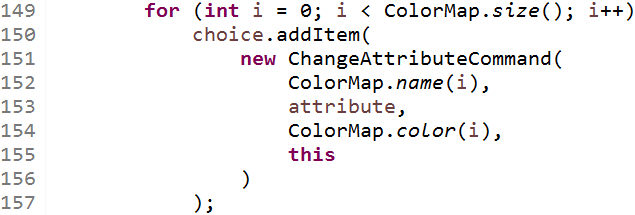
\includegraphics[width=\linewidth]{multipleLine/pic2-1}
%\caption{Nested interval example.}
%  \label{fig:pic2-1}
%\end{figure}

%\begin{figure}[H]
%\centering
%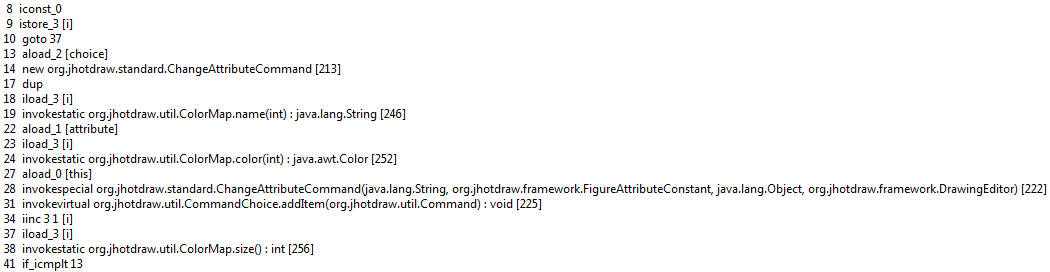
\includegraphics[width=\linewidth]{multipleLine/pic2-2}
%\caption{Bytecode to \figref{pic2-1}.}
%  \label{fig:pic2-2}
%\end{figure}

%\begin{figure}[H]
%\centering
%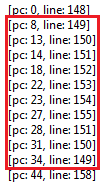
\includegraphics[width=0.3\linewidth]{multipleLine/pic2-3}
%\caption{Line number table/interval to \figref{pic2-1}.}
%  \label{fig:pic2-3}
%\end{figure}

Neither in bytecode nor in line number attribute we can extract the exact interval of method invocations. Generally, we cannot distinguish if the interval represents a method invocation or a loop. Another interesting thing is that in the figure multiple corresponding pcs are included.
\lt{change to scntactic example}
\renewcommand\lstlistingname{Code}
\begin{Java}[caption={Incomplete interval example.}, label={code:5-1}, firstnumber=22]
fooTestSupporter
	.bla(getObject(),
		staticMethod(o),
		fooTestSupporter2.bla2(null,
			o));
\end{Java}

\renewcommand\lstlistingname{Bytecode}
\begin{JVMIS}[caption={Bytecode to \coderef{5-1}.}, label={code:5-2}, breaklines=true]
18  aload_1 [fooTestSupporter]
19  invokestatic isFieldOrLocalVariableNullExample.testMethodCall.FooTest.getObject() : java.lang.Object [26]
22  aload_3 [o]
23  invokestatic isFieldOrLocalVariableNullExample.testMethodCall.FooTest.staticMethod(java.lang.Object) : java.lang.Object [30]
26  aload_2 [fooTestSupporter2]
27  aconst_null
28  aload_3 [o]
29  invokevirtual isFieldOrLocalVariableNullExample.testMethodCall.FooTestSupporter.bla2(java.lang.Object, java.lang.Object) : java.lang.Object [34]
32  invokevirtual isFieldOrLocalVariableNullExample.testMethodCall.FooTestSupporter.bla(java.lang.Object, java.lang.Object, java.lang.Object) : void [38]
\end{JVMIS}

\begin{JVMIS}[caption={Line number table/interval to \coderef{5-1}.}, label={code:5-3}, breaklines=true]
[pc: 18, line: 22]
[pc: 19, line: 23]
[pc: 22, line: 24]
[pc: 26, line: 25]
[pc: 28, line: 26]
[pc: 29, line: 25]
[pc: 32, line: 23]
\end{JVMIS}


%\begin{figure}[H]
%\centering
%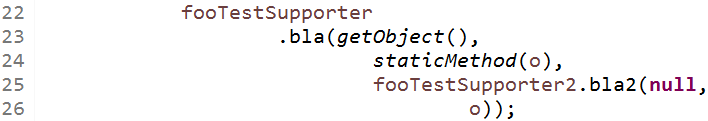
\includegraphics[width=\linewidth]{multipleLine/pic5-1}
%\caption{Incomplete interval example.}
%  \label{fig:pic5-1}
%\end{figure}

%\begin{figure}[H]
%\centering
%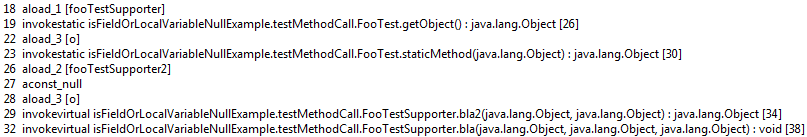
\includegraphics[width=\linewidth]{multipleLine/pic5-2}
%\caption{Bytecode to \figref{pic5-1}.}
%  \label{fig:pic5-2}
%\end{figure}

%\begin{figure}[H]
%\centering
%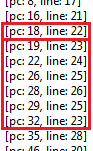
\includegraphics[width=0.3\linewidth]{multipleLine/pic5-3}
%\caption{Line number table/interval to \figref{pic5-1}.}
%  \label{fig:pic5-3}
%\end{figure}

By using the algorithm we only get the interval from pc 19-32, but actually pc 18 also belongs to the interval. That the missing pc is missing will be detected in step 4\&5 when traversing back the ArrayList by the number of parameters. If it is not a static method invocation and there is not enough possible method receivers stored in that ArrayList to traverse back, the missing pc is added in retrospect.

\renewcommand\lstlistingname{Pseudocode}
\begin{Java}[caption={Multiple line interval algorithm.}, label={alg:multipleLineAlg}]
i = index in line number attribute which contains the invoke.* opcode

if (lineNrAttribute[j>i] <= lineNrAttribute[i]) {	
			
	if (isAlternating(i,j))
		return getAlternatingInterval(i, j);
		
	// non-alternating
	b = j which has the smallest line number after j;
	a = corresponding index to b; // index<k which has the same line number as b||k
	return getNonAlternatingInterval(a, b);	
	
} else if (lineNrAttribute[j<i] == lineNrAttribute[i]) {

		b = i;
		a = j;
		return getInterval(a, b);
		
}	
\end{Java}

This pseudocode will give a very rough idea how the invocation interval can be read out. The detailed implementation can be seen in the classes \code{MultipleLineManager}\footnote{\label{package2}In package \emph{ch.unibe.scg.nullSpy.instrumentator.controller.methodInvocation}.} and \code{MethodInvocationAnalyzer}\textsuperscript{\ref{package2}}.

\subsection{Obtaining Variable Data Difficulties - Fields}
\label{subsec:variableDifficulties}
We previously mentioned that NullSpy first collects data about fields and we met some difficulties regarding this. By using the method \code{loopBody()} from class \code{Javassist.expt.ExprEditor} (\subsecref{fields}) for gathering information caused those troubles because it loops through the GIVEN \code{methodInfo} which contains the bytecode sequence of a method. Even after finding a field assignment and adding some additional bytecode to it, the method still iterates through the unchanged \code{methodInfo} it got as parameter without the additional bytecode. Getting the right start-pc of a field assignment is not a straight forward process as it may seem.

After entered extra instructions the method \code{loopBody()} iterates onwards until it finds a key which indicates an access to a field. Normally, Javassist provides a method with which the start-pc of the field access can be find out easily, but in our case not due to bytecode alternation. This method returns the start-pc of the field as if there was no changes, however it actually has to return a bigger start-pc than it does. The start-pc is needed to distinguish in what category the field has to be assigned to (\subsecref{fields}).

To find the right start-pc of the field assignment, we compare the start-pc returned by a method of Javassist with the \code{afterStorePc} of the previously found field assignment. Every time an assignment is found we store it as a reference for the next assignment to obtain the right data. Even for the store-pc of an assignment (\textit{``put.*"} the last found field is essential. If there is more interest how those pcs are obtained, please see the class \code{FieldAnalyzer}\footnote{In package \emph{ch.unibe.scg.nullSpy.instrumentator.controller}.}.

\subsection{Bytecode Adaptation Difficulties}
\label{subsec:bytecodeAdaptationDifficulties}
The reason why we decided to use Javassist for our NullSpy project is because the thought of only using the source-level API \figref{bytecodeModificationLevels} to implement everything. It would have been much easier to only operate at source-level instead of learning how to read bytecode or extract data from it or enter extra code into it, yet at the end we still had to do everything at bytecode-level.

One big problem encountered while inserting the test method between an assignment and a closing bracket \code{\}}. We tried to insert additional code as shown in \figref{insertionCodeExample} by specifying the exact line number where it should be entered in source code. Unfortunately Javassist first checks the specified line whether it contains some code (only symbols excluded). If there is no code at that line it computes the next line that contains some and inserts the test method right before it. Please visualize a situation where for example a local variable is created/instantiated at the end of a \code{if-body}. In this situation Javassist adds the extra code right before the next code line which is outside the existing scope of the local variable.

\renewcommand\lstlistingname{Code}
\begin{Java}[caption={Bytecode adaptation example.}, label={code:bytecodeAdaptationExample_1}]
Object fontName;
if (fName.startsWith("A")) {
	fontName = new Arial();
} else {
	fontName = new Calibri();
}
\end{Java}

\begin{Java}[caption={Wrong Adaptation to \coderef{bytecodeAdaptationExample_1}.}, label={code:bytecodeAdaptionExample_2}]
Object fontName;
if (fName.startsWith("A")) {
	fontName = new Arial();
 } else {
	--<inserted code which takes ``fontName'' as parameter>--
	fontName = new Calibri();
}
\end{Java}


That is why changed the way to insert the test method at bytecode-level. Like this we first have to build up the bytecode sequence and then enter it before a specific pc. Please take a look at the class \code{ByteCodeAdapter}\footnote{In package \emph{ch.unibe.scg.nullSpy.instrumentator.controller}.} how the bytecode sequence is created.

There are of course many other small problems during the implementation of NullSpy but these mentioned are the most troublesome ones.

\section{Limitations}
\label{sec:limitations}
During the implementation of NullSpy we had to change the concept few times due to limitations or an overhead that could have grown immense.

Our first idea of how NullSpy could track the NullPointerExceptions is to gather information about variable assignment, which is the case now, and also inject another test method right before each method invocations. In small projects this way could have worked fine but in larger projects which could contain hundreds of classes with a lot of method invocations the execution time would be strongly influenced.

Being able to collect data about variables we still are not able to avoid injecting bytecode even it affects the runtime. Related to this issue a limitation about Javassist is mentioned before namely inserting bytecode right before a closing bracket (\subsecref{bytecodeAdaptationDifficulties}). Because of this it highly depends on the location where additional code should be inserted whether using the source-level API is possible or not. \ugh{Avoiding checking all the location where something new should be added it is more secure to do this on bytecode-level.}\lt{ändern} But in cases like entering something at the beginning or at the end of a method body the source-level is just fine.

Another limitation of Javassist to mention is that it does not provide anything to get information about method receivers. It only allows one to extract information about local variables, fields and method invocations itself. The programming language Java also does not provide any information about the method receiver, since the exception object or the stack trace element only contains the class, file, method name and the line number. Nonetheless making possible to gather data about them the algorithm discussed before (see \algref{methodReceiverAlg}) fulfills the missing task.

The last limitation we want to discuss here is that unfortunately NullSpy is not capable to track the root of NullPointerExceptions that are originated in a null which was returned of a method call or in an element of a collection. Why those situations are not supported in NullSpy is because of the impossibility way to store them, e.g. imagine a nested ArrayList or a HashMap and a never ending return value of method invocations. So we lack something tangible to compare with each other, get a hit and read the location out of the hit (\secref{futureWork}).

\chapter{Validation}
\label{ch:validation}
This chapter will provide some numbers to compare the execution time each project takes, the original and the instrumented one. To get the numbers we instrumented the example project JHotDraw. 

\section{JHotDraw}
\label{sec:jhotdraw}
{JHotDraw\footnote{\protect\url{http://www.jhotdraw.org/}}} also served to check whether the logic of the bytecode manipulation behind NullSpy is working as desired. JHotDraw is an open-source Java GUI framework for technical and structured Graphics. It is big enough to get reliable numbers and it provides many different cases we had to take care of in NullSpy. Also thanks to Nevena Milojkovi\'{c} and her experience with the combination Javassist and JHotDraw we as well decided to test NullSpy on it.

\section{Execution Time Difference}
\label{sec:execTimeDiff}
How did we get the numbers? First of all, of course another executable jar file of the modified project has to be created. The steps to it are followings: load project, modify project, store modified project, build project that creates an executable jar file of the original project and one of the modified one. We then simulate the terminal with a Java class to run each jar thirty times and calculate the average. The next table lists each execution time and the average:

\begin{table}[H]
\centering
\begin{tabular}{ l | S[table-format=1.3] | S[table-format=1.3]|}
\cline{2-3}	  &\textbf{Original project} & \textbf{Modified project}\\ \cline{2-3}
	1	& 7.223	& 7.442	\\ \cline{2-3}
	2	& 7.427	& 7.738	\\ \cline{2-3}
	3	& 7.171	& 7.893	\\ \cline{2-3}
	4	& 7.035	& 7.379	\\ \cline{2-3}
	5	& 7.488	& 7.458	\\ \cline{2-3}
	6	& 7.194	& 7.691	\\ \cline{2-3}
	7	& 6.849	& 7.472	\\ \cline{2-3}
	8	& 7.286	& 8.068	\\ \cline{2-3}
	9	& 7.083	& 7.519	\\ \cline{2-3}
	10 & 7.27	& 7.55	\\ \cline{2-3}
	11 & 7.16	& 7.177 \\ \cline{2-3}
	12 & 7.161  & 7.55	\\ \cline{2-3}
	13 & 7.225	& 7.223	\\ \cline{2-3}
	14 & 7.037	& 7.316	\\ \cline{2-3}
	15 & 7.067	& 7.54	\\ \cline{2-3}
	16 & 6.975	& 7.77	\\ \cline{2-3}
	17 & 7.287	& 7.117	\\ \cline{2-3}
	18 & 7.52	  & 7.488	\\ \cline{2-3}
	19 & 7.303	& 7.35	\\ \cline{2-3}
	20 & 6.942	& 7.307	\\ \cline{2-3}
	21 & 7.147	& 7.535	\\ \cline{2-3}
	22 & 7.222	& 7.644	\\ \cline{2-3}
	23 & 7.145	& 7.32	\\ \cline{2-3}
	24 & 7.334	& 8.187	\\ \cline{2-3}
	25 & 7.364	&7.488	\\ \cline{2-3}
	26 & 7.269	&7.942	\\ \cline{2-3}
	27 & 7.441	&7.943	\\ \cline{2-3}
	28 & 7.223	&7.467	\\ \cline{2-3}
	29 & 6.912	&7.647	\\ \cline{2-3}
	30 & 7.363	&7.784	\\ \cline{2-3}
	\cline{2-3}
	\end{tabular}
	\caption{Execution time.}
	\label{tab:executionTime}
\end{table}

\begin{table}[H]
	\centering
	\begin{tabular}{ | S[table-format=1.4] | S[table-format=1.6] |}
		\hline	
		\textbf{Original project} & \textbf{Modified project}\\ \hline
		7.2041	&	7.566834 \\
		\hline
	\end{tabular}
	\caption{Average time.}
	\label{tab:averageTime}
\end{table}

The runtime of the modified project takes 0.362734s longer than the original one, this means after adding additional code to the project results in approximately \textbf{5\%} overhead. This small overhead is quite negligible. But this numbers have to be interpreted with caution because the overhead is only measured on JHotDraw.

\chapter {Conclusion and Future Work}
\label{ch:conclusionFutureWork}
Now we have come so far to retrospect (step back and have a critical loot at) the entire project for summarizing what goals we have achieved so far and for proposing further aims that could be completed in the future. In a small section we also want to talk about the gained experience during the whole project.

\section{NullSpy}
\label{sec:nullSpy}
Happily, we could say here that we successfully managed to meet the main purpose we have set at the beginning of the project. NullSpy is now capable to tracking the NullPointerExceptions to its root and provide the user with more information about its origin without spending much time on finding it. The most important steps which lead to the success of NullSpy are listed below:

\begin{enumerate}
\item Extract and gather information about all method receivers because method invocations on these causes NullPointerExcetptions. To achieve this, we developed an algorithm (\algref{methodReceiverAlg}) with the function of finding method receivers and extracting data from it by only doing static bytecode analysis. The information about it is then stored as an external csv file. It is needed for a comparison in in a later step.

\item Again collecting data, but this time about variable assignments namely local variables and fields. Here next to the static bytecode analysis additional instructions are inserted to the class files to check right after the assignment if the variable is assigned to the special value \code{null}. If this is the case everything about the variable is stored in a HashMap which serves for a comparison too. It is stored in a HashMap because if a variable is assigned to another object than null, it will be deleted from the HashMap.

\item NullSpy does only handle the uncaught NullPointerException which means we can wrap up the main method with a catch block. In this catch block the class name and the line number where the NullPointerException occurred is extracted from the stack trace. This information is passed to a method in which the parameter helps to find the guilty method receiver. With the hit the exact location where that variable was set to null can be derived from the HashMap.

\item All the additional needed classes are added to the project after it is modified and stored in a folder the user has chosen. Being able to run the modified project of course a jar file is created. In our case JHotDraw already provides a \textit{build.xml} which we had to alternate a little bit.
\end{enumerate}

During the implementation we were encountered with many difficulties. Some of those we were able to solve and some not unfortunately. Those unsolved ones could be proposed as goals of future work. The next section will list some of them.

\section{Future Work}
\label{sec:futureWork}
\subsection{Support unsupported method receivers and variable assignments}
As mentioned in (\secref{limitations}), if the cause of a NullPointerException lies in an element of a collection or in an object that is returned by a method invocation, it cannot be tracked to its assignment location. Come up with a way to extract and store information could be a future aim. Of course gathering information about the method receivers has to be improved too.

\subsection{Track NullPointerException root for all projects}
As now our goal in this project was tracking null assignments of JHotDraw. First of all, we had to make sure that building JHotDraw works properly with the additional classes. To fulfil this task manual changes on the build.xml was necessary. If this can be done automatically by NullSpy it would be much better.

Next to this we only looked at the assignment and method receiver types which appear in JHotDraw itself. There could be other types that are not covered in NullSpy depending on projects. In case NullSpy is used on projects that contain not supported issues improving it to cover them can be added to the toDo list.

\subsection{Plug-in for Eclipse}
Last target for future work to mention here is transform NullSpy into an Eclipse compatible plug-in project. After integrated it with Eclipse the null tracking can be started without any expenses on how to manipulate the build.xml if there is one or even bother to create an executable jar file out of it.

For now, we can only think of these future work that could improve NullSpy to give it more value.

\section{Personal Experience}
At the beginning, after reading the description of the project I had no clue how to approach its goal at all. Since this is my first big project on my own but with help from two experienced research assistants I learned a lot, especially in the matter of programming.

As the project is all about manipulating class files, here with Javassist, we first had to learn how bytecode is constructed and get familiar with Javassist. Luckily there is a very good tutorial that teaches one how to use it. This class library however does not cover everything we needed. Thanks to this we had to deal with the lack extensively and learned quite a lot about working on bytecode-level.

Next to getting familiar with bytecode we also had to invent algorithms like that of extracting method receivers from the bytecode or that of getting the pc interval of a method receiver. It was quite interesting to invent those as these are the first ones that fulfill more complex tasks.

Debugging: It is not as easy as it seems. Sometimes it took hours to find the cause of a small bug, and after fixing it another occurs. The reason why it took that long to debug is because along with checking whether the logic of our code was right we also had to find the right bytecode position to ensure the implementation does what it is created for.

Coding beautifully the way so that it will not smell was another challenge due to lack of experience. Sometimes I tended to put everything in one class instead of abiding by the single responsibility principle. Therefore, refactoring the whole project multiple times was necessarily which also took some time. Best before starting to code is to clearly thinking through what is needed, how the structure should look like and what kind of responsibility each class of the project should take for gaining time for other things.

We also came in contact with the building XML file and the jar file. Concerning the XML file, we gained experience by learning a new language by modifying it that it also creates a jar file out of the modified project. 

\chapter {Anleitung zu wissenschaftlichen Arbeiten}
NullSpy is a program which helps Java developers to find the root of NullPointerExceptions by providing an additional link next to the common stack trace. The key idea behind NullSpy is to help developers to save time fixing bugs which are caused by NullPointerExcpetions. Of course this approach tries to provide this service by keeping the overhead to a minimum. To demonstrate how NullSpy works, this chapter serves as a small tutorial that takes JHotDraw as the testing project to show the feature of NullSpy.

\section{Installation}
\label{sec:installation}
For this tutorial JHotDraw is needed. In order to download it, visit the following site and download ``JHotDraw6.0 beta 1" (version we worked with during the implementation of NullSpy):\\
\href{http://www.jhotdraw.org}{www.jhotdraw.org}\\
Unpack the archive and store it to a location of your choice. To be able to run JHotDraw additional libraries are used, that are not included in JHotDraw itself. Following libraries are to be downloaded:\\
``batik-all-1.7": \href{http://www.java2s.com/Code/Jar/b/Downloadbatikall17jar.htm}{www.java2s.com/Code/Jar/b/Downloadbatikall17jar}\\
``jdo": \href{http://www.java2s.com/Code/Jar/j/Downloadjdojar.htm}{www.java2s.com/Code/Jar/j/Downloadjdojar}\\
Again unpack those archives and store them in a lib folder in your JHodDraw project.

Running the tests of JHotdraw with the commando line the location of libraries ``hamcrest" and ``junit" are needed, which are normally also downloaded when the programming environment Eclipse\footnote{Can be downloaded here: \href{https://eclipse.org/downloads/}{www.eclipse.org/downloads}} is downloaded.





%END Doc
%-------------------------------------------------------

\bibliography{scg}
\bibliographystyle{plain}

\clearpage
\thispagestyle{empty}
\null\vfill
\begin{center}
''Ich erkl\"are hiermit, dass ich diese Arbeit selbstst\"andig verfasst und  keine  anderen  als  die  angegebenen  Quellen  benutzt  habe. 
Alle Stellen, die w\"ortlich oder sinngem\"ass aus Quellen entnommen  wurden,  habe  ich  als  solche  gekennzeichnet.  Mir  ist  bekannt,  dass  andernfalls  der  Senat  gem\"ass  Artikel 36  Absatz 1 Buchstabe 
r  des  Gesetzes  vom  5. September 1996  \"uber  die  Universit\"at zum Entzug des auf  Grund dieser Arbeit verliehenen Titels berechtigt ist.“
\end{center}
\vfill
\clearpage

\end{document}